\section{LTI-Systeme}{171}

\begin{tabular}{ll}
    $x(t)$                  & Eingangssignal \\
    $y(t)$                  & Ausgangssignal \\
    $\delta(t)$             & Dirac-Stoss \\
    $h(t)$                  & Impulsantwort (Antwort auf Dirac-Stoss) \\
    $H(\jimg \omega)$       & Frequenzgang \\
    $|H(\jimg \omega)|$     & Amplitudengang \\
    $\theta(\jimg \omega)$  & Phasengang \\
    $H(s)$                  & $H(s) = \frac{Y(s)}{X(s)}$ Übertragungsfunktion (UTF)
\end{tabular}


\subsection{Zusammenhänge zwischen den Grössen}{174-176}
\label{Zusammenhang}

Die Impulsantwort $h(t)$ und der Frequenzgang $H(\jimg \omega)$ sind ein \\
\textbf{Fourier-Transformationspaar}:

\begin{center}
    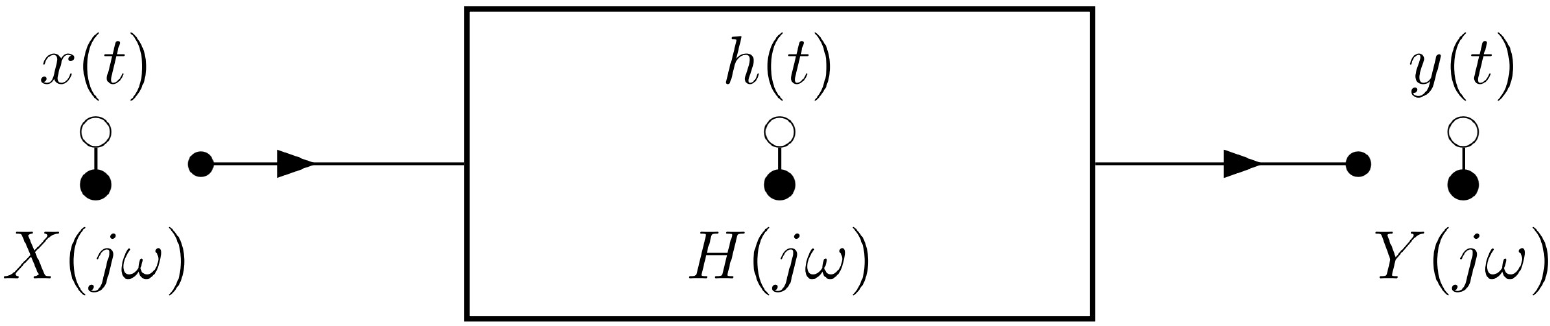
\includegraphics[width=0.7\columnwidth]{images/frequenzgang_impulsantwort.png} \\
\end{center}

Die Impulsantwort $h(t)$ und die Übertragungsfunktion $H(s)$ sind ein\\
\textbf{Laplace-Transformationspaar}:
$$ \boxed{ h(t) \, \laplace \, H(s) } $$

Das Ausgangssignal berechnet sich als: 
$$ \boxed{ y(t) = h(t) * x(t) \, \laplace \, Y(s) = H(s) \cdot X(s) } $$


\subsubsection{Zusammenhang Impulsantwort -- Einheitssprungantwort}

\begin{tabular}{ll}
    $h(t)$ & Impulsantwort \\
    $g(t)$ & Einheitssprungantwort
\end{tabular}

$$ \boxed{ h(t) =  \frac{\diff g(t)}{\diff t}  \quad \Leftrightarrow \quad g(t) = \int\limits_{-\infty}^t  h(\tau) \, \diff \tau }  $$
$$ \boxed{ H(s) = s \cdot G(s) \quad \Leftrightarrow \quad G(s) =  \frac{1}{s} H(s) }  $$


\subsubsection{Zusammenhang Impulsantwort \& Kausalität LTI-System}

\fbox{\parbox{0.9\linewidth}{
Damit ein LTI-System kausal ist, muss dessen Impulsantwort $h(t)$ für alle $t < 0$ gleich Null sein. 
} }


\subsection{Phasenlaufzeit \texorpdfstring{$\tau_P(\omega)$}{tP(w)}}{183}
Die Phasenlaufzeit ist nur für \textbf{reine Sinus-Schwingungen} exakt bestimmbar! \\
Das System ist beschrieben durch:

$$ x(t) = A \cdot \sin(\omega_0 t + \gamma) $$
$$ H( \jimg \omega) = \alpha \cdot e^{- \jimg  \omega t_0} \, \laplace \, h(t) = \alpha \cdot \delta(t - t_0) $$


Das Ausgangssignal $y(t) = x(t) * h(t)$ ist gegenüber dem Eingangssignal $x(t)$ mit Faktor $\alpha$ gewichtet und 
um die Zeit $t_0$ verzögert. \\
\textrightarrow\ \textbf{Diese Verzögerung wird Phasenlaufzeit genannt}
$$ \boxed{ \tau_P(\omega) = \frac{- \theta(\omega)}{\omega} } $$

$ \theta(\omega)$ entspricht dem Phasengang des Systems 


\example{Phasenlaufzeit}

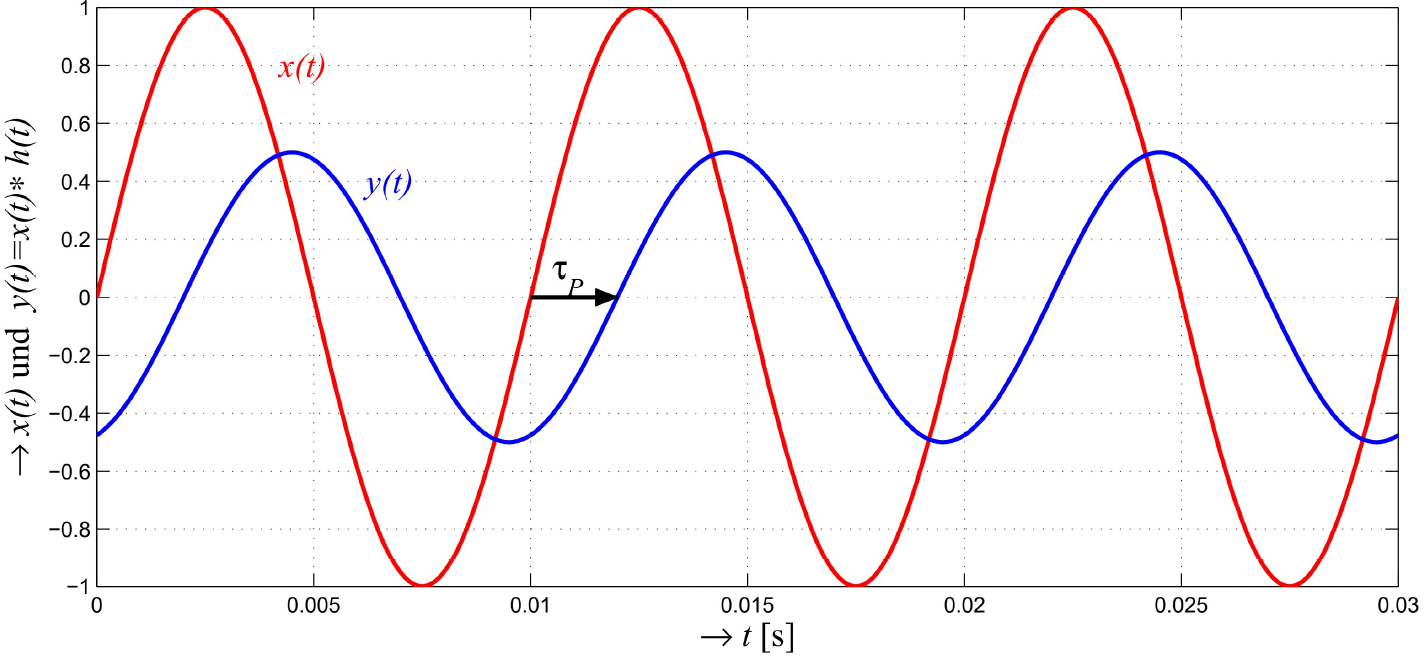
\includegraphics[width=0.8\linewidth]{images/phasenlaufzeit.png}


\subsubsection{Negative Phasenlaufzeit}

Eine negative Phasenlaufzeit bedeutet \textbf{nicht}, dass ein System \textbf{akausal} ist!


\subsection{Gruppenlaufzeit \texorpdfstring{$\tau_G(\omega)$}{tG(w)} }{182}

Definiert für Signale mit \textbf{mehreren Frequenzanteilen}\medskip

Bei amplitudenmodulierten Signalen bestimmt die Gruppenlaufzeit $\tau_G(\omega)$ die \textbf{Verzögerung der Hüllkurve} der AM.

$$ \boxed{ \tau_G(\omega) = \frac{-\diff \theta(\omega)}{\diff \omega} } $$

$\theta(\omega)$ entspricht dem Phasengang des Systems\medskip

Die Gruppenlaufzeit kann nur dann als \textbf{Laufzeit des Signals} interpretiert werden, wenn im Frequenzbereich des Signales 
die Gruppenlaufzeit und auch die Dämpfung ungefähr konstant sind.


\subsubsection{Negative Gruppenlaufzeit}

Bei \textbf{Vierpolen} mit \textbf{konzentrierten Elementen} ist in bestimmten Frequenzbereichen eine 
\textbf{negative Gruppenlaufzeit} möglich, insbesondere in Frequenzbereichen wo die Dämpfung stark ändert.
(z.B. Nullstellen der UTF) 

Bei negativer Gruppenlaufzeit erscheint die Wirkung \textbf{nicht} vor der Ursache! \\
\textrightarrow\ Das System ist \textbf{nicht} akausal! \\
Das Maximum der Hüllkurve am Ausgang kann aber \textbf{früher} als am Eingang auftreten.


\subsection{Phasenlaufzeit / Gruppenlaufzeit identisch}{186}\label{Phasenlaufzeit / Gruppenlaufzeit identisch}

Die \textbf{Signalverzögernug, Phasenlaufzeit} $\tau_P(\omega)$ und \textbf{Gruppenlaufzeit} 
$\tau_G(\omega)$ sind identisch, wenn
$$ \boxed{ \theta(\omega) = - \omega \cdot t_0  } $$

und der \textbf{Amplitudengang ebenfalls konstant} ist, d.h. $H(j \omega) = \alpha \cdot e^{-j \omega t_0}$ \\
Die Signalverzögerung beträgt für \textbf{alle Frequenzen} $t_0 \, (= \tau_P = \tau_G) $ 


\subsection{Verzerrungen}{187-188}

Stimmt der zeitliche Verlauf einer Schwingung auf der Empfängerseite nicht mehr mit der Senderseite überein, arbeitet das
Übertragungssystem \textbf{nicht verzerrungsfrei}.


\subsubsection{Lineare Verzerrung}

Eine \textbf{Dämpfung} eines Signals (z.B. durch einen Tiefpassfilter) entspricht einer \textbf{linearen Verzerrung}


\subsubsection{Nichtlineare Verzerrung}

Nichtlineare Verzerrungen werden durch \textbf{Übersteuerung} des Systems \textbf{(Kanal)} oder dessen
\textbf{nichtlineare Kennlinie} hervorgerufen. \\
Durch nichtlineare Verzerrungen treten \textbf{neue}, im Ursprungssignal nicht enthaltene \textbf{Schwingungen} auf.\\
Ein \textbf{Mass} für nichtlineare Verzerrungen ist der \textbf{Klirrfaktor}


\subsection{Klirrfaktor}{189}

Verhältnis des \textbf{Effektivwerts} der \textbf{neu} am Ausgang eines Systems entstandenen \textbf{Harmonischen} zum 
Effektivwert des gesamten Signals

\begin{minipage}[b]{0.48\columnwidth}
    $$ \boxed{ k = \sqrt{\frac{U_2^2 + U_3^2 + \cdots + U_n^2}{U_1^2 + U_2^2 + \cdots + U_n^2}}} $$
\end{minipage}
\hfill
\begin{minipage}[c]{0.48\columnwidth}
    \raggedright%
    $U_1$ entspricht der Grundharmonischen\\
    \textrightarrow\ Es gilt: $1 > k \geq 0$
\end{minipage}


\subsubsection{Klirrdämpfungsmass}

$$ \boxed{ a_k = 20 \cdot \log_{10} \Big( \frac{1}{k}  \Big)  } $$


\subsubsection{Total Harmonic Distortion (THD)}
Wird vor allem im englisch-sprachigen Raum verwendet

\begin{minipage}[b]{0.48\columnwidth}
   $$ \boxed{  \text{THD} = \sqrt{\frac{U_2^2 + U_3^2 + \cdots + U_n^2}{U_1^2} } } $$
\end{minipage}
\hfill
\begin{minipage}[c]{0.48\columnwidth}
    \raggedright%
    $U_1$ entspricht der Grundharmonischen\\
    \textrightarrow\ Es gilt:  $\infty > \text{THD} \geq 0$ 
\end{minipage}

\vspace{0.2cm}
geringe Verzerrungen: $\text{THD} \approx k$ \qquad allgemein: $\text{THD} > k$


\subsection{Verzerrungsfreie Übertragung von Signalen}{190}

Frequenzgang $H(j \omega)$ und Impulsantwort $h(t)$ eines verzerrungsfreien Signals:

$$ \boxed{ H(\jimg  \omega) = \alpha \cdot e^{- \jimg  \omega t_0} 
    = | H(\jimg  \omega)|  \cdot e^{\jimg  \theta(\omega)}  \, \laplace \,  h(t) = \alpha \cdot \delta(t - t_0) } $$


Damit ein Signal verzerrungsfrei übertragen wird, müssen folgende Bedingungen erfüllt sein:

\begin{enumerate}
    \item \textbf{Amplitude} konstant (unabhängig von der Frequenz) \textlrarrow\ $| H(\jimg  \omega)| = \text{konstant} = \alpha \neq 0$\\
        \textrightarrow\ Keine Amplitudenverzerrung vorhanden
    \item \textbf{Phase} proportional zur Frequenz \textlrarrow\ $\theta(\omega) = - \omega \, t_0$\\
        (äquivalenz zu Abschnitt\ \ref{Phasenlaufzeit / Gruppenlaufzeit identisch})
        \textrightarrow\ Keine Phasenverzerrung vorhanden
\end{enumerate}


\subsection{Übertragung stochastischer Signale}{193-194}

Wird ein stochastisches Signal $x(t)$ (schwach stationär) durch ein LTI-System mit Impulsantowort $h(t)$ übertragen, so berechnet
sich das Ausgangssignal $y(t)$ gemäss Abschnitt\ \ref{Zusammenhang} aus:

$$ \boxed{ y(t) = h(t) * x(t) = \int\limits_{- \infty}^{\infty} x(\tau) \, h(t - \tau) \, \diff \tau  \, 
\laplace \, Y(s) = H(s) \cdot X(s) } $$


\subsubsection{Linearer Mittelwert}

Der lineare Mittelwert $Y_0$ des Ausgangssignals $y(t)$ bei der Frequenz $\omega = 0$ entspricht

% mathematisch semi korrekt...
$$ \boxed{ Y( \jimg \omega = 0) = Y(\jimg 0) = X(\jimg 0) \cdot H(\jimg 0) \Rightarrow Y_0 = X_0 \cdot H(\jimg 0) } $$

$H(\jimg  \omega)$ = Frequenzgang und $X_0$ = linearer Mittelwert von $x(t)$ 


\subsubsection{Autokorrelationsfunktion (AKF) des Ausgangssignals}

Da $\varphi_{yy}(\tau)$ und $Y_0$ nicht von $t$ abhängen, ist auch $y(t)$ schwach stationär.

$$ \boxed{ \varphi_{yy}(\tau) = \int\limits_{- \infty}^{\infty} \int\limits_{- \infty}^{\infty} h(\alpha) \, h(\beta) \, \varphi_{xx}(\tau + \alpha - \beta) \, \diff \alpha \, \diff \beta 
= h(-\tau) * h(\tau) * \varphi_{xx}(\tau) } $$

Es gelten folgende Zusammenhänge für die Fourier-Transformationspaare:

\begin{ctabular}{O M O | O M O}
    h(-\tau) & \laplace\ & H^*(\jimg  \omega)     & \varphi_{xx}(\tau) & \laplace\ & \Phi_{xx}(\jimg  \omega) \\
    h(\tau)  & \laplace\ & H(\jimg  \omega)       & h(\tau) * h(-\tau) & \laplace\ & \abs{H(\jimg  \omega)}^{2}
\end{ctabular}


\subsubsection{Leistungsdichtespektrum (PSD)}

Die AKF und das PSD sind ein Fourier-Transformationspaar
$$ \underbrace{\varphi_{yy}(\tau)}_{\text{AKF}} \, \laplace \, \underbrace{\Phi_{yy}(\jimg  \omega)}_{\text{PSD}} $$

Daraus folgt der Zusammenhang der Leistungsdichtespektren $\Phi(j \omega)$
$$ \boxed{ \Phi_{yy}(\jimg  \omega) = |H(j \omega)|^2 \, \Phi_{xx}(\jimg  \omega) } $$

Für die AKF des Ausgangssignals $y(t)$ gilt 
$$ \boxed{ \varphi_{yy}(\tau) = \frac{1}{2 \pi} \int\limits_{- \infty}^{\infty} |H(\jimg  \omega)|^2 \, \Phi_{xx}(\jimg  \omega) \, e^{\jimg  \omega \tau} \diff \omega } $$

Die Leistung $Y^2$ des Ausgangssignals $y(t)$ berechnet sich beim Zeitpunkt $\tau = 0$ als
$$ \boxed{ Y^2 = \varphi_{yy}(0) = \frac{1}{2 \pi} \int\limits_{- \infty}^{\infty} |H(\jimg  \omega)|^2 \, \Phi_{xx}(\jimg  \omega) \, \diff \omega } $$


\subsubsection{Kreuzkorrelationen}

Die Kreuzkorrelationsfunktionen $\varphi_{xy}(\tau)$ und $\varphi_{yx}(\tau)$ des stochastischen, reellen Eingangssignals $x(t)$ 
(Klasse 2b) und des stochastischen Ausgangssignals $y(t)$ eines LTI-Systems hängen folgendermassen zusammen:

$$ \boxed{ \varphi_{xy}(\tau) = h(\tau) * \varphi_{xx}(\tau) \, \laplace \, \Phi_{xy}(\jimg  \omega) = H(\jimg  \omega) \cdot \Phi_{xx}(\jimg  \omega) } $$
$$ \boxed{ \varphi_{yx}(\tau) = h(-\tau) * \varphi_{xx}(\tau) \, \laplace \, \Phi_{yx}(\jimg  \omega) = H^*(\jimg  \omega) \cdot \Phi_{xx}(\jimg  \omega) } $$

Somit gilt:
$$ \boxed{ \varphi_{yx}(\tau) = \varphi_{xy}(-\tau) \, \laplace \, \Phi_{yx}(\jimg  \omega) = \Phi_{xy}(-\jimg  \omega) = \Phi^*_{xy}(\jimg  \omega) } $$

